%\documentclass[hyperref={pdfpagelabels=false}]{beamer}
\documentclass[handout]{beamer}

\usetheme{Heidelberg}

\usepackage{wrapfig}
\usepackage{lmodern}
\usepackage{natbib}
\usepackage{amsmath,amsfonts,amssymb}
\usepackage{algorithm,algorithmic}

\usepackage{natbib}

%\usepackage{tikz}
%	\usetikzlibrary[topaths,arrows,calc]
%\usepackage{wrapfig}
\usepackage{graphicx}
%\usepackage{stackengine}
\usepackage{subcaption}
\captionsetup[subfigure]{labelformat=empty}


\usepackage[english]{babel}
\usepackage[T1]{fontenc} % Ligaturen, richtige Umlaute im PDF 
\usepackage[utf8]{inputenc}% UTF8-Kodierung für Umlaute usw

\usepackage{hyperref}

\definecolor{darkred}{rgb}{110,1,1}  
\definecolor{maroon}{rgb}{0.5,0,0}  

\newcounter{saveenumi}
\newcommand{\seti}{\setcounter{saveenumi}{\value{enumi}}}
\newcommand{\conti}{\setcounter{enumi}{\value{saveenumi}}}


% zusaetzlich ist das usepackage{beamerthemeshadow} eingebunden 
\usepackage{beamerthemeshadow}

\renewcommand{\thefootnote}{\fnsymbol{footnote}} 

%--------------------------------------------------------------------------%
%--------------------------------------------------------------------------%
\def\vec{\mathop{\rm vec}}								% matrix vectorization
\def\tr{\mathop{\rm tr}}								% matrix trace
\def\argmax{\mathop{\rm argmax}}						% argmax
\def\argmin{\mathop{\rm argmin}}						% argmin
\def\median{\mathop{\rm median}} 						% median
\def\dist{\mathop{\rm dist}} 						    % dist
%--------------------------------------------------------------------------%
%--------------------------------------------------------------------------%
%--------------------------------------------------------------------------%
\begin{document}

\begin{frame}
\frametitle{Agenda}
\tableofcontents
\end{frame} 
%--------------------------------------------------------------------------%
%--------------------------------------------------------------------------%
\section{Graph matching} 
\subsection{Introduction}

\begin{frame}
\frametitle{Attributed undirected graph}
Attributed undirected graph $G=(V,E,D)$
\begin{itemize}
\item set of nodes $V=\{v_i\}_{i=1}^{n}$
\item set of edges $E\subseteq\{\{u,v\}| u, v\in V\}$
\item node attributes $D=\{d_i\}_{i=1}^{n}$, $D\subset\mathbb{R}^r$
\end{itemize}
\vspace{1cm}
\begin{figure}[b]
    \centering
    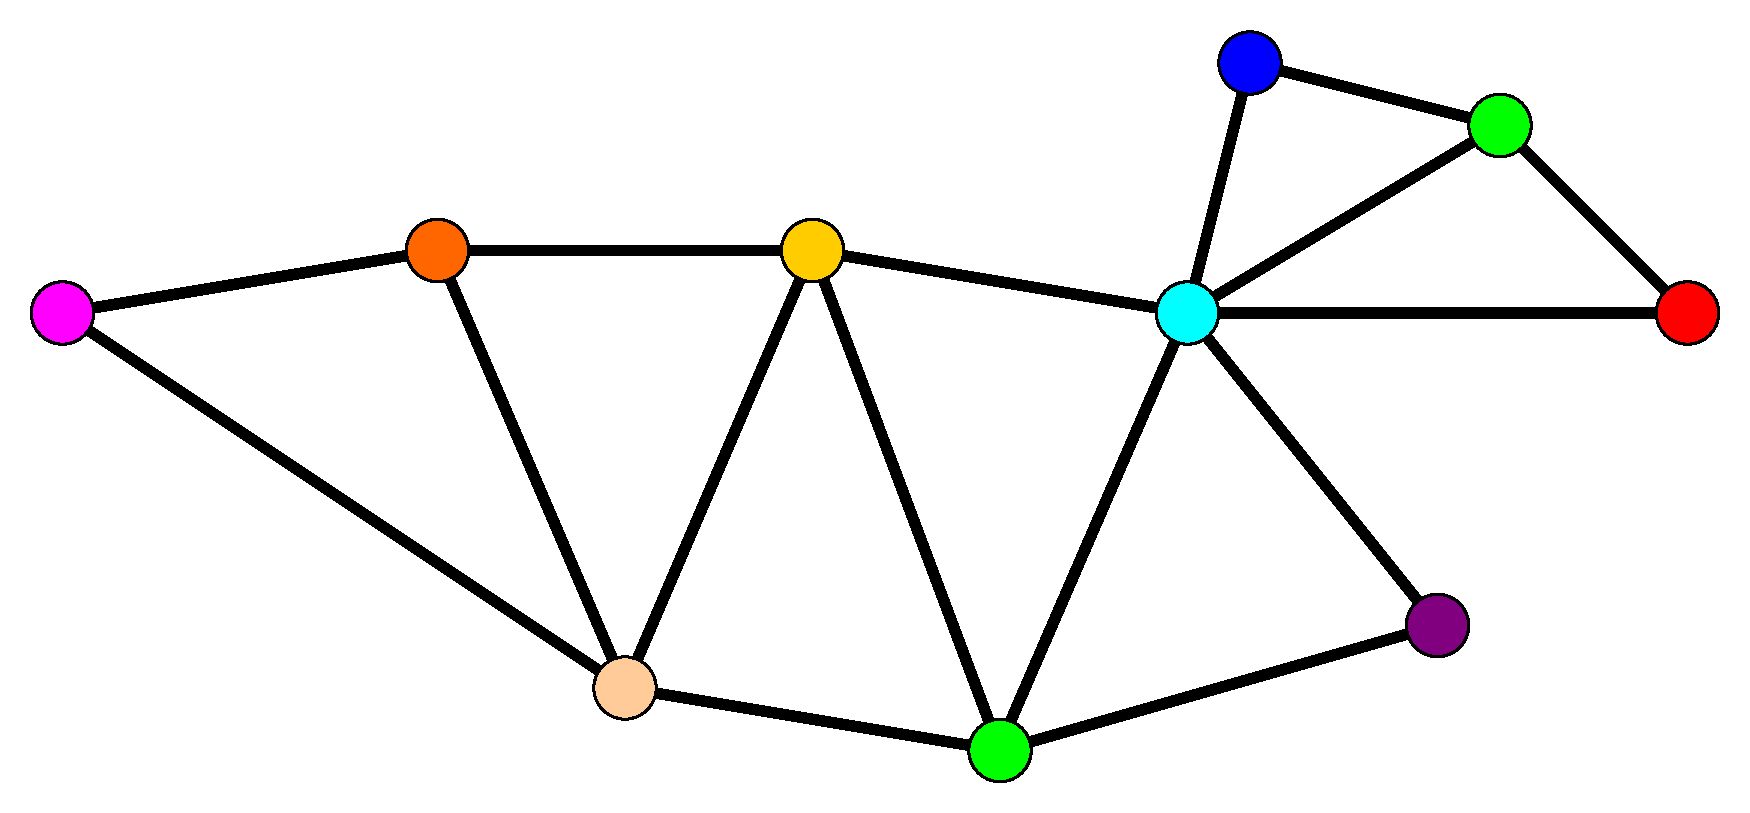
\includegraphics[width=5cm]{fig/at_graph_1.pdf}
\end{figure}%
\end{frame}
%--------------------------------------------------------------------------%
\subsection{Graph matching}
\begin{frame}
\frametitle{Graph matching}
Let us consider two undirected attributed graphs $G^I = (V^I, E^I, D^I)$ and $G^J = (V^J, E^J,D^J)$: % with $|V^I|=n_1$ and $|V^J|=n_2$:
\begin{figure}[t]
        \centering
        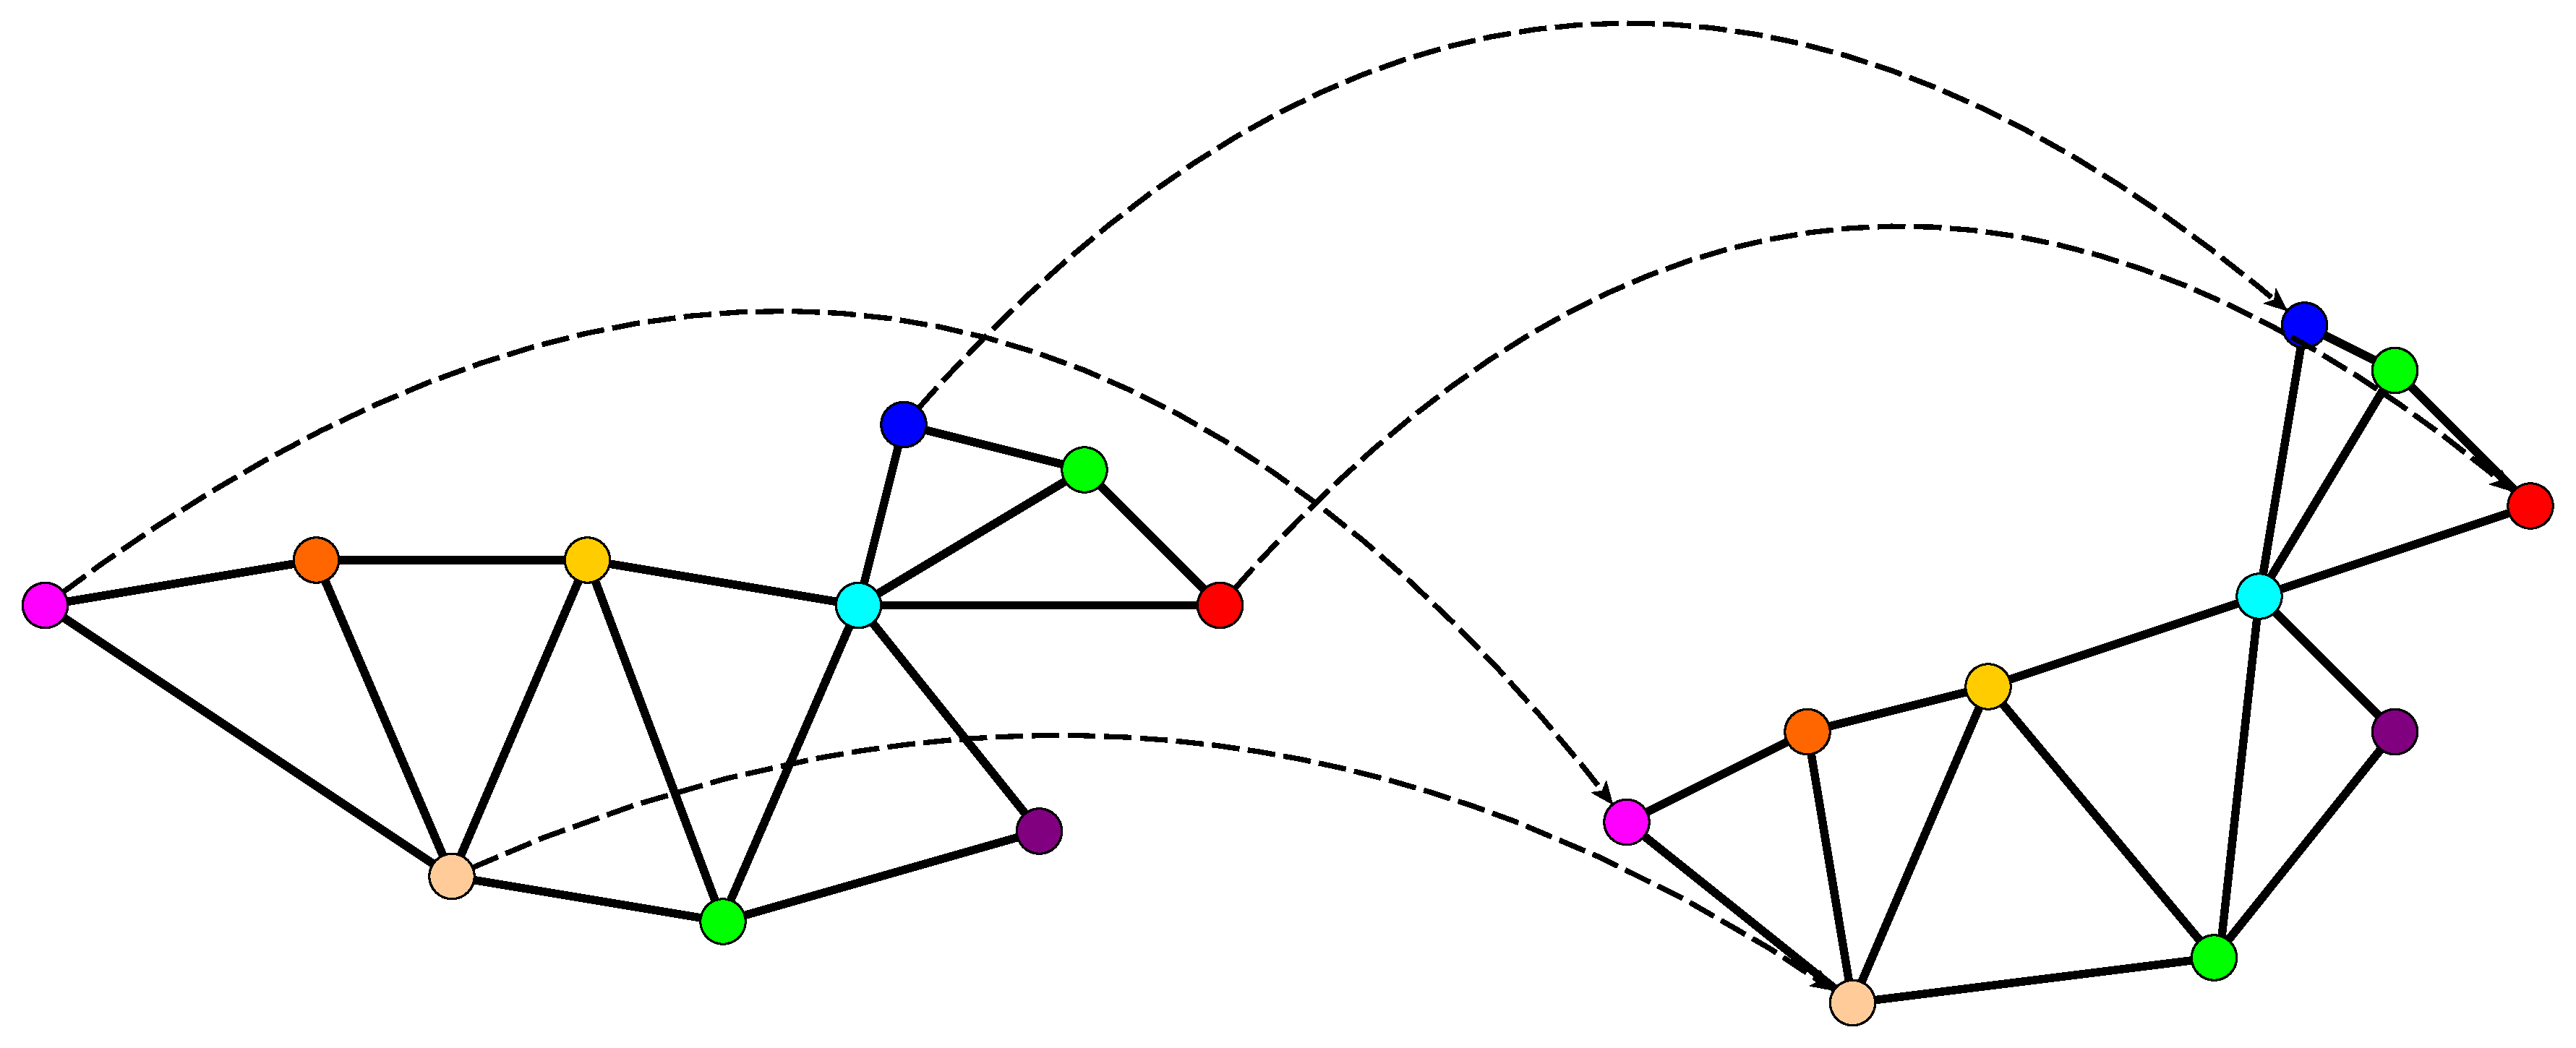
\includegraphics[width=5cm]{fig/matching_12.pdf}
\end{figure}
A matching function between $G^I$ and $G^J$ is a mapping %between the sets of nodes of two graphs:
\\
{\hspace{4cm}$m:V^I\rightarrow V^J$}\textcolor{red}{\hspace{2cm}not unique!}

Define a function $S(G^I, G^J, m)$ to measure the quality of matching $m$ that fulfills some constraints\\
$\Rightarrow$ \textcolor{red}{Graph matching problem} between $G^I$ and $G^J$ 
\begin{equation*}
m = \argmax_{\hat{m}}S(G^I, G^J, \hat{m})
\end{equation*}

\end{frame}
%--------------------------------------------------------------------------%
\begin{frame}
\frametitle{Graph matching in computer vision}
\begin{figure}[t]
    \centering
    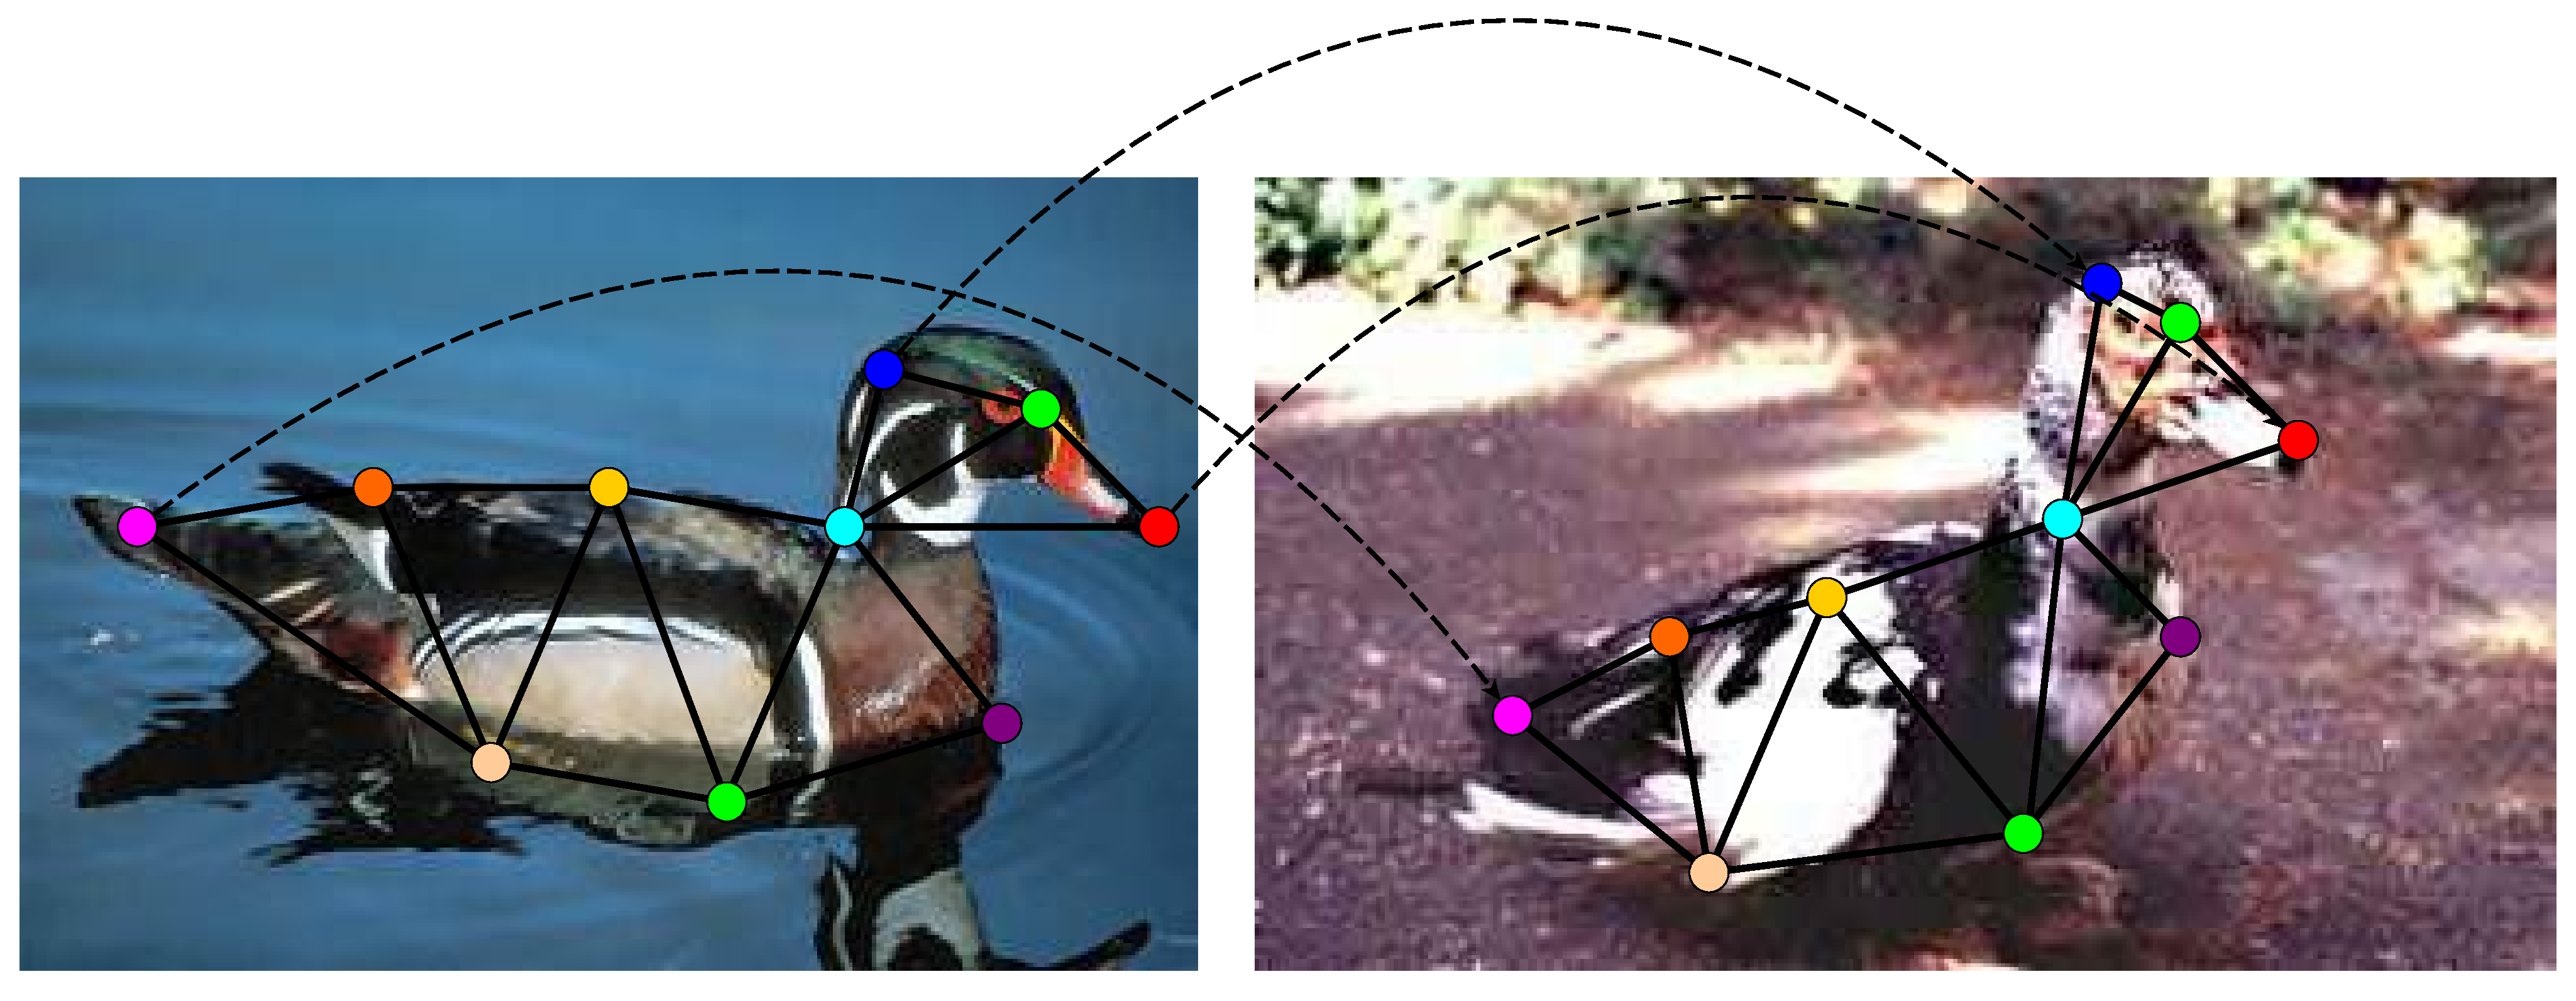
\includegraphics[width=5cm]{fig/ducks_12.pdf}
\end{figure}
\begin{itemize}
\item image matching
\item shape matching
\item object detection
\item object tracking
\item $\dots$
\end{itemize}
\end{frame}
%--------------------------------------------------------------------------%
\begin{frame}
\frametitle{Graph matching}
A matching function between $G^I$ and $G^J$ is a mapping %between the sets of nodes of two graphs:
\\
{\hspace{4cm}$m:V^I\rightarrow V^J$}

Graph matching problem between $G^I$ and $G^J$ 
\begin{equation*}
m = \argmax_{\hat{m}}S(G^I, G^J, \hat{m})
\end{equation*}


Depending on the required properties of a matching one distinguishes
\begin{itemize}
\item exact graph matching
\item inexact graph matching
\end{itemize}

\end{frame}
%--------------------------------------------------------------------------%
\subsection{Exact graph matching}
\begin{frame}[allowframebreaks]
\frametitle{Exact graph matching}
Edge preserving mapping $m$:
$\{v_i,v_{i^\prime}\}\in E^I\Rightarrow\{m(v),m(v_{i^\prime})\}\in E^J$ % for all $v_i,v_{i^\prime}\in V^I$.

\vspace{10pt}
\begin{minipage}[0.2\textheight]{\textwidth}
	\begin{columns}[T]
		\begin{column}{0.6\textwidth}
			\begin{itemize}
			\item mapping $m$ is bijective $\rightarrow$ graph isomorphism (GI)
			\end{itemize}
		\end{column}
		\begin{column}{0.3\textwidth}
			{\tiny subgraph isomorphism, maximal common subgraphs}
		\end{column}
	\end{columns}
\end{minipage}

\vspace{10pt}
\begin{minipage}[0.2\textheight]{\textwidth}
	\begin{columns}[T]
		\begin{column}{0.6\textwidth}
			\begin{itemize}
			\item mapping $m$ is injective $\rightarrow$ graph monomorphism
			\end{itemize}
		\end{column}
		\begin{column}{0.3\textwidth}
			{\tiny second graph can contain additional nodes and edges}
		\end{column}
	\end{columns}
\end{minipage}

\vspace{10pt}
\begin{minipage}[0.2\textheight]{\textwidth}
	\begin{columns}[T]
		\begin{column}{0.6\textwidth}
			\begin{itemize}
			\item mapping $m$ is total\hspace{15pt} $\rightarrow$ graph homomorphism
			\end{itemize}
		\end{column}
		\begin{column}{0.3\textwidth}
			{\tiny every node has to be mapped}
		\end{column}
	\end{columns}
\end{minipage}

\vspace{10pt}
\textcolor{red}{NP complete (except GI)~{\tiny\citep{Garey_NPComplet}}}

\framebreak
%--------------------------------------------------------------------------%
Exact graph matching:
\begin{itemize}
\item too strict
\item time/memory consuming
\item cannot handle object deformation
\end{itemize}
\begin{figure}[htb]
	\centering
	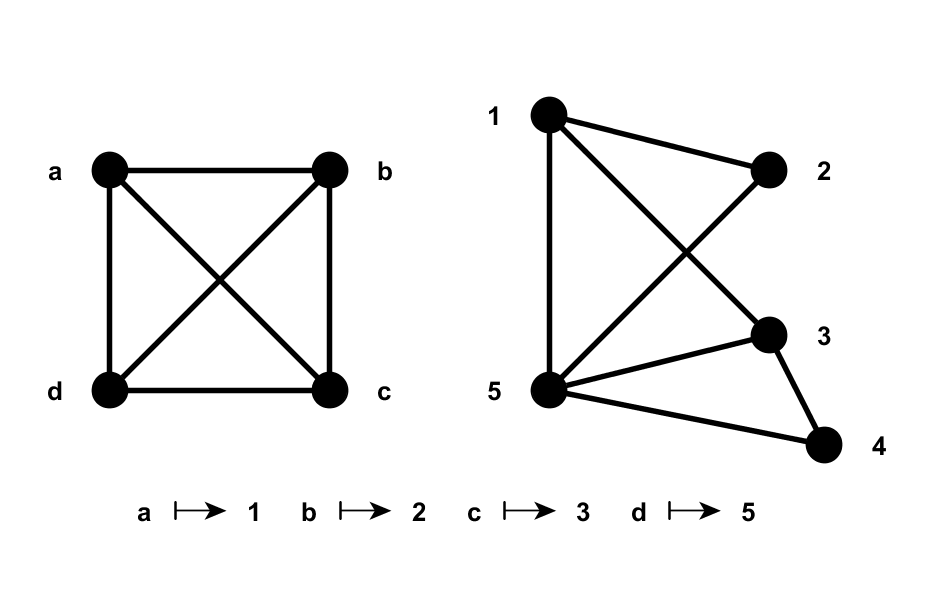
\includegraphics[width=0.5\textwidth]{fig/inexactGM}
\end{figure}
\end{frame}

%--------------------------------------------------------------------------%
\subsection{Inexact graph matching}
\begin{frame} [allowframebreaks]
\frametitle{Inexact graph matching}
Introduce similarity measure between nodes/edges in the graphs
%Do not require exact correspondences between two graphs
\begin{equation*}
m = \argmax_{\hat{m}}S(G^I, G^J, \hat{m})
\end{equation*}
\begin{itemize}
\item second-order (edge) similarity \textcolor{red}{$s_E(e_{ii^\prime},e_{jj^\prime})$}, $e_{ii^\prime}\in E^I, e_{jj^\prime}\in E^J$
\item first-order (node) similarity \textcolor{red}{$s_V(v_{i},v_{j})$}, $v_i\in V^I, v_j\in V^J$
\end{itemize}

\begin{equation*}
	S(G^I,G^J,m)=\sum_{\substack{m(v_i)=v_j\\m(v_i^{\prime})=v_j^{\prime}}}s_E(e_{ii^\prime},e_{jj^\prime}) + \sum_{m(v_i)=v_j}s_V(v_{i},v_{j})
\end{equation*}

\begin{itemize}
\item assignment matrix $X\in\{0,1\}^{n_1\times n_2},\ X_{ij}=1\iff m(v_i)=v_j$ \\
      vector form $x = \vec{X}$
\end{itemize}

\framebreak
The most common problem formulation:
\begin{block}{Quadratic Assignment Problem (NP complete)~{\tiny\citep{Burkard98thequadratic}}}
$$x^* = \arg\max \sum_{\substack{x_{ij}=1\\x_{i^\prime j^\prime}=1}}s_E(e_{ii^\prime},e_{jj^\prime}) + \sum_{x_{ij}=1}s_V(v_{i},v_{j}) $$
$$ s.t. \begin{cases}
		x\in\{0,1\}^{n_1n_2} \\
		\sum_{i=1}^{n_1}x_{ij}\le 1 \\
		\sum_{j=1}^{n_2}x_{ij}\le 1
\end{cases}$$
\end{block}
Using matrix notation : $\arg\max_{x}{x^TSx}$, $S$ is a similarity (or affinity) matrix

%Algorithms that solve this problem can be optimal or suboptimal.

\framebreak

Solution techniques
\begin{itemize}
\item discrete optimization
	\begin{itemize}
	\item tree search~{\tiny tree search with backtracking}
	\item simulated annealing~{\tiny}
	\end{itemize} 
\item continuous optimization
	\begin{itemize}
		\item constraint relaxation~{\tiny\ Frank-Wolfe Algorithm, search direction by linear assignment problem}
		\item spectral methods~{\tiny eigenvalue decomposition of adjacency matrices, only graph geometry}
		\item probabilistic frameworks~{\tiny optimal assignment between set of labels and set of objects; EM: nodes
				of the first graph are considered as an observed data and the nodes of the second
				graph as hidden random variables}
		\item clustering~{\tiny agglomerative clustering+threshold the cluster size; additional constraints, complexity reduction, set of independent problems}
	\end{itemize} 
\end{itemize}
\end{frame}
%--------------------------------------------------------------------------%
\begin{frame}
\frametitle{Drawback of the existing algorithms}

\begin{itemize}
\item most of the algorithms are developed for matching relatively small graphs ($\sim 150$ nodes)
\item scale badly due to the polynomial increase of time and storage demand
\item algorithms for the big graphs use another formulation of the graph matching optimization problem\\
\vspace{5pt}
{\centering
$x^* = \argmin_{X}\|A^I-XA^JX^T\|^2+\|D^I-XD^J\|^2_2$}
\end{itemize}

\end{frame}
%--------------------------------------------------------------------------%
\begin{frame}
\frametitle{Aim of the master's thesis}
\begin{itemize}
\item a novel framework that should help to extend the usability
of existing graph matching algorithms to bigger graphs
\item a variant of the well-known divide and conquer paradigm:\\
	subdividing initial problem into a set of smaller problems, which can be easily handled with existing algorithms
\item iterative algorithm that allows to improve initial subdivision into subproblems
\end{itemize}

\end{frame}
%--------------------------------------------------------------------------%
%--------------------------------------------------------------------------%
\section{Two level graph matching framework (2LevelGM)}

\begin{frame}
\frametitle{Complexity reduction}
\begin{block}{}
\tiny
$$x^* = \arg\max x^TSx $$
$$ s.t. \begin{cases}
		x\in\{0,1\}^{n_1n_2} \\
		\sum_{i=1}^{n_1}x_{ij}\le 1 \\
		\sum_{j=1}^{n_2}x_{ij}\le 1
\end{cases}$$
\end{block}

\begin{itemize}
\item set of candidate correspondences~{\tiny replace initial problem with one smaller problem}
\item sparse affinity matrix
\item subdivide problem into a set of smaller subproblems
\hspace{10pt}\textcolor{red}{$\leftarrow$\\}
Similar works:
			\begin{itemize}
				\item semisupervised case~{\tiny spectral co-clustering}
				\item another objective function~{\tiny minimization, relaxation labeling}
				\item special kind of subproblem~{\tiny cluster = direct neighborhood of a node}
			\end{itemize}
\end{itemize}
\end{frame}
%--------------------------------------------------------------------------%
\begin{frame}
\frametitle{Two level graph matching framework}
Lower level: initial graphs $G^I$, $G^J$\\
Higher level: simplified graphs (anchor graphs $A^I$, $A^J$)\\
\begin{enumerate}
\item find correspondences between nodes of the anchors graphs (higher level);
\item find for each pair of matched anchors a mapping between the nodes of the
underlying subgraphs (lower level);
\item updates subgraphs;
\item runs further through steps 1 and 3 until no improvement in
the overall solution is achieved in several successive iterations.
\end{enumerate}
\end{frame}
%--------------------------------------------------------------------------%
\begin{frame}
\frametitle{Anchor graph construction}
Goal: $G^I=(V^I,E^I, D^I)\rightarrow A^I=(V^{Ia},E^{Ia},U^{Ia})$

Equivalent: partitioning of $G^I\supset(G^I_1\cup\dots\cup G^I_{|V^{Ia}|})$

Done by: \begin{itemize}
			\item grid with $r$ rows and $c$ columns
			\item multi-level graph partitioning algorithms, 3 phases
		\end{itemize}
\end{frame}
%--------------------------------------------------------------------------%
\begin{frame}
\frametitle{Anchor graph and subgraph matching}
Goal: find correspondences between two anchor graphs $A^I=(V^{Ia},E^{Ia},U^{Ia})$ and $A^J=(V^{Ja},E^{Ja},U^{Ja})$

\begin{itemize}
	\item edge similarity: compare length of the edges beween anchors
	\item node similarity: 
	\begin{itemize}
		\item score of the matching of $G^I_k$ and $G^J_p$
		\item bag of features model
		\item each histogram represents a distribution of
		the length of the subgraph edges inside a small circle region around a node
		\item $\chi^2$ statistic test
	\end{itemize}
\end{itemize}

Match anchor graphs and subgraph using some existing algorithm (e.g.~RRWM)
\end{frame}

%--------------------------------------------------------------------------%
\begin{frame}
\frametitle{Graph partition update}
\begin{enumerate}
\item two affine transformations $T_{kp}:V^I_k\rightarrow V^J_p$ and $T_{pk}:V^J_p\rightarrow V^I_k$(point set registration problem)
\item transformation $T_{pk}$ is casted as $T_{pk}:V^J_p\rightarrow V^I$

 projected points $T_{pk}(v_j) \rightarrow$ nearest neighbors $\bar{v}_i=NN(T_{pk}(v_j))$ 
 
 a new matrix $\bar{U}^{Ia}\in\mathbb{R}^{|V^I|\times m_1}$ 
 
 $\bar{U}^{Ia}_{\bar{v}_i,a_k}=\|T_{pk}(v_j)-\bar{v}_i\|_2$ the distance between the projections and their nearest neighbor.
\end{enumerate}
%\begin{figure} [h]
%	\centering
%	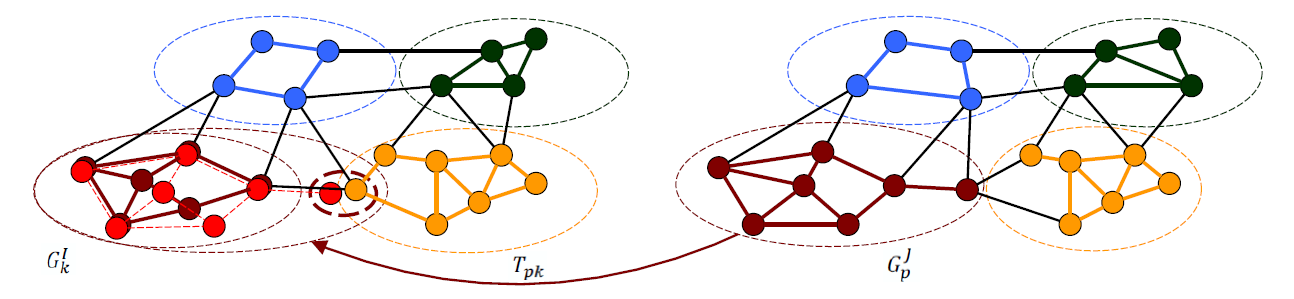
\includegraphics[scale=0.35]{fig/2levelGM/update.png}
%\end{figure}
\end{frame}
%--------------------------------------------------------------------------%
%\begin{frame}
%\frametitle{Complexity}
%%complexity of a selected graph matching algorithm $\mathcal{O}(f_{GM}(n_1,n_2))$
%\begin{itemize}
%%\item Graph partitioning: $\mathcal{O}(n_2^2)$ 
%%\item Codebook of node attributes: 
%\item size of the anchor graphs and subgraphs
%\item number of iterations
%\end{itemize}
%\end{frame}
%--------------------------------------------------------------------------%
%--------------------------------------------------------------------------%
\section{Evaluation} 
\begin{frame}
\frametitle{Evaluation}
%\centering 
%{\Huge Evaluation}
Two ways of evaluation have been used
\begin{itemize}
\item synthetic data
\item real data
\end{itemize}

Accuracy -> recall: number of correct detected matches divided by the number of all correct matches
\end{frame}

\subsection{Synthetic data}
\begin{frame}[allowframebreaks]
\frametitle{Synthetic data}
\textbf{Performance of the 2LevelGM with non-attributed anchor graphs}

To our best knowledge, those algorithms have not been applied directly to graphs with more than $150$ nodes each without additional problem simplifications 

\begin{enumerate}
\item the SM algorithm has the worst matching quality in all cases

\item 2LevelGM performs a little bit unstable. The average performance of 2LevelGM is a little bit lower than the one of IPFP and RRWM, although in individual runs 2LevelGM is not worse.

\item The running time of 2LevelGM is slower as of IPFP and RRWM. 

\item The slowest algorithm in this comparison is MPM. 

\item Nevertheless MPM achieved  best accuracy and objective score in three of four tests. It is outperformed by 2LevelGM in the first test with significantly smaller time demand

\end{enumerate}

\framebreak

\textbf{Performance of the 2LevelGM with attributed anchor graphs}

geometrical structure of the subgraphs

the size of histograms: $35$ bins

radius $R$ of the circle region around each node: $2$

\begin{enumerate}
\item  direct improved performance time of the 2LevelGM algorithm in all tests.

\item a more stable performance in the second test. 

\item be more susceptible to graph deformations: selected anchor attributes are not sufficiently robust against deformations in the length of edges.
\end{enumerate}
\framebreak
{\small
\textbf{Comparison of 2LevelGM, GLAG and PATH on bigger graphs}

\begin{enumerate}
\item GLAG, PATH another optimization problem => can be directly applied to bigger graphs without the necessity to reduce the set of possible candidate matches; initialized with the weighted adjacency matrices
\item do not provide averaged results for this group of tests due to their high computational demand
\item all tests for bigger graphs can be considered as instances of the graph isomorphism problem in exact (1 line) and inexact (2,3 line).

\item 2LevelGM outperforms both GLAG and PATH in objective score and especially in running time with one exception

\item Overall 2LevelGM shows a high matching accuracy in all three tests. 

\item Additionally we believe it is possible to improve the framework by solving instability issues, which we saw in previous cases. 
\end{enumerate}

}

\end{frame}
%--------------------------------------------------------------------------%
\subsection{Real data}
\begin{frame}[allowframebreaks]
\frametitle{Image affine transformation}
\small
$152$ MSER keypoints

\begin{enumerate}
\item 2LevelGM is able to find the absolutely correct matching for the whole set except one image pair and therefore shows better results in objective score and accuracy than ProgGM, PATH and GLAG.

\item The result of matching of the last image pair is roughly the same for 2LevelGM and ProgGM. We notice that 2LevelGM is not able to improve graph partitioning further in this case,

\item ProgGM is the fastest algorithm in this comparison. 2LevelGM is a little bit slower than ProgGM. However ProgGM directly stops as soon as the matching score does not increase any more. In contrast to that, our 2LevelGM has to make some additional iterations at the end to ensure that a local minimum is found. This is done intentionally, as we cannot make certain statements about the convergence of our framework.
\end{enumerate}
\end{frame}
%--------------------------------------------------------------------------%
\begin{frame} %[allowframebreaks]
\frametitle{House data set}
\small
\begin{enumerate}
\item $111$ images of a toy house taken from different viewpoints
\item around $250$ MSER keypoints on each image
\item provided ground truth is extrapolated (extrapolation radius $10$)
\item 2LevelGM: grid initialization with $2\times 2$ cells + codebook of features
\item ProgGM shows better matching accuracy
\item simple feature matching and GLAG have the lowest accuracy
\item PATH shows the third best result. more robust against deformations
\item running time of 2LevelGM and ProgGM lie in the same range
\item 2LevelGM is comparable with ProgGM for small values of the sequence gap
\item Reasons: RRWM and ineffectiveness of our update rule to improve graph partitions
\end{enumerate}

\end{frame}
%--------------------------------------------------------------------------%
%--------------------------------------------------------------------------%
\begin{frame}{The end}
\centering
\LARGE
\color{red}
Thank you for your attention!
\end{frame}
%--------------------------------------------------------------------------%

\end{document}
%--------------------------------------------------------------------------%
%--------------------------------------------------------------------------%
%--------------------------------------------------------------------------%
